\chapter{Fundamentos sensores remotos}

Esta clase tiene como objetivo familiarizarze con el entorno gráfico del \emph{SNAP}. El \emph{SNAP (Sentinel Aplication Toolbox)} es un  software de procesamiento de imágenes diseñado por la \emph{Agencia Espacial Europea (ESA)}, cuyas herramientas simplifican el trabajo con imágenes radar y ópticas.

Durante el curso se trabajará con imágenes de la región de triple frontera, que incluye el límite entre la provincia de Misiones, en Argentina, Brasil y Paraguay.

En esta zona (Figura \ref{fig:mapa}) se encuentra los Parques Nacionales Iguazú (Argentino) e Iguaçu (Brasil), el aeropuerto internacional de cataratas del Iguazú, los rios Iguazú, frontera entre Argentina y Brasil, y Parana, frontera entre Paraguay y Argentina, las ciudades de Foz de Iguaçu (Brasil), iudad del Este (Paraguay) y Puerto Iguazú (Argentina), el embalse Ugugua-Í

\begin{figure}[h!]
    \centering
    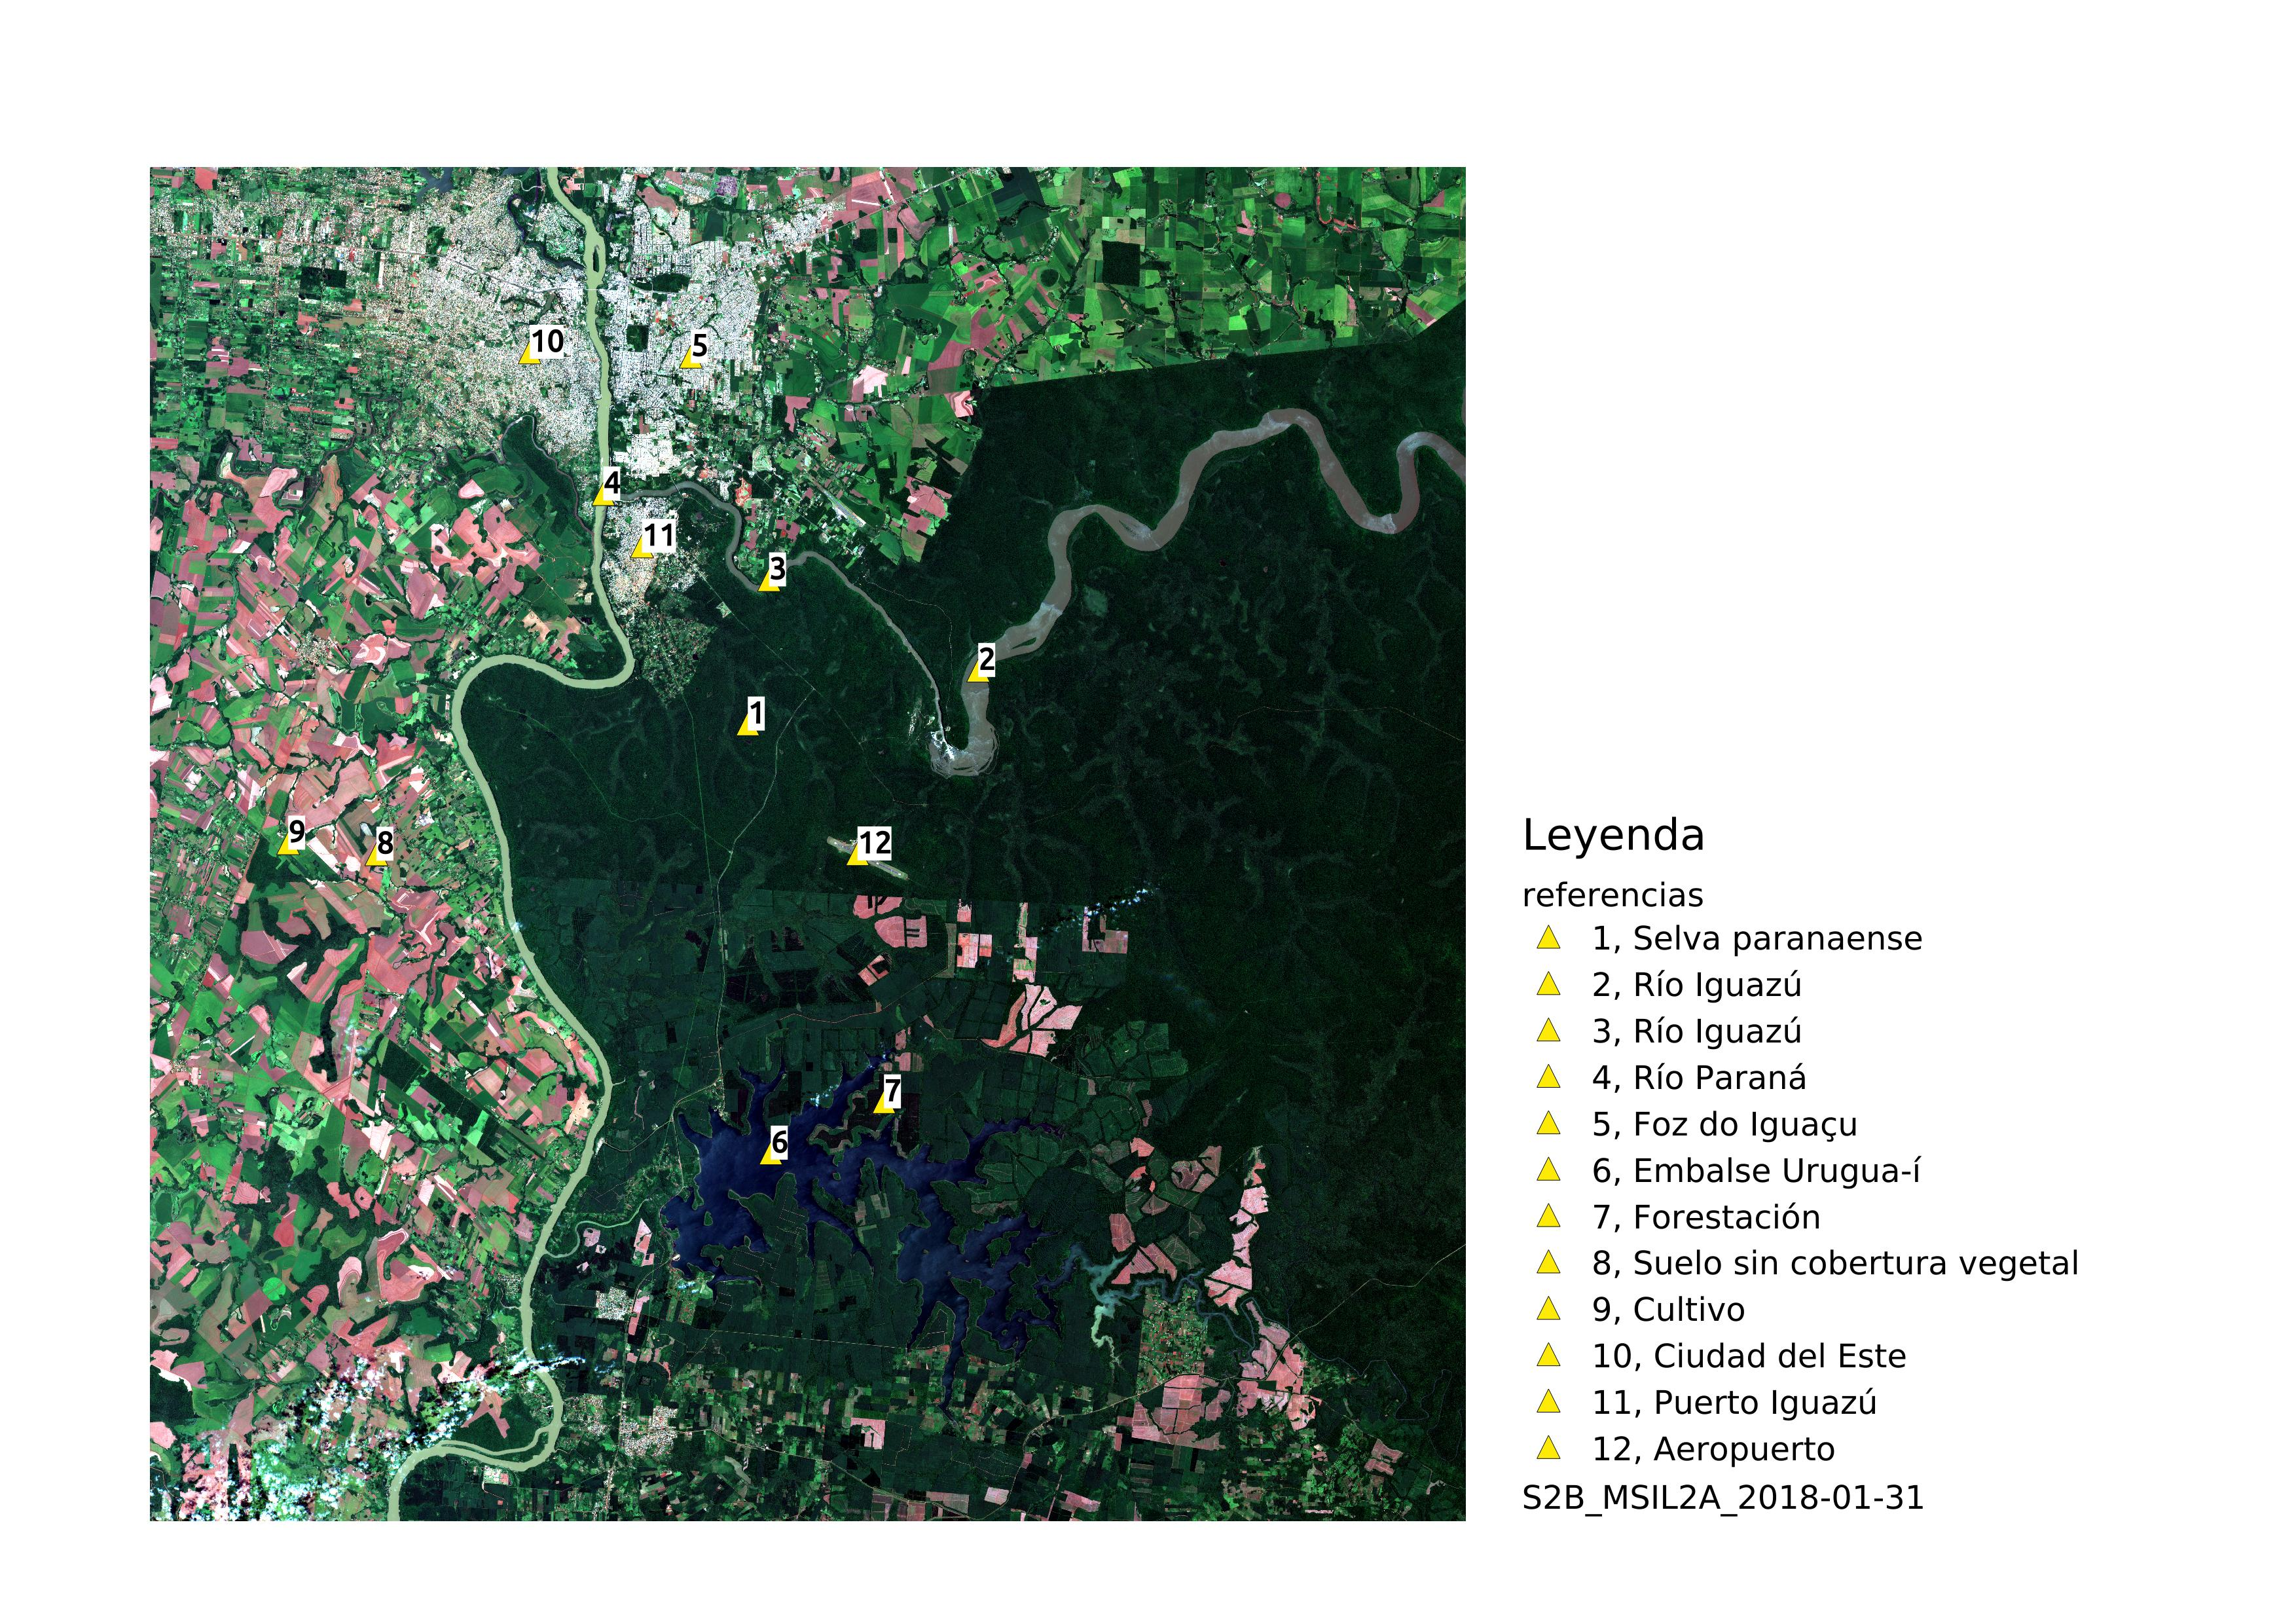
\includegraphics[width=0.7\textwidth]{fig:mapa.jpg}
    \caption{Mapa de la zona de triple frontera.}
    \label{fig:mapa}
\end{figure}

\section{Sobre esta guía}

A lo largo de la guía usaremos como referencia:

\begin{itemize}
  \item \menu{Archivo>Abrir...} para indicar una ruta en el menú de un programa o una herramienta.
  \item \directory{Documentos/archivo.doc} para indicar una carpeta o archivo dentro de una carpeta.
  \item \texttt{Opción} para indicar una opción de configuración de un programa.
  \item \keys{ctrl + c} para indicar una combinación de teclas.
  \item \emph{SAR} para indicar un termino específico o importante para la clase.
\end{itemize}

Además las rutas estarán siempre definidas a partir de la carpeta \directory{material}.

\section{Interfaz gráfica del SNAP}

Descomprima el archivo \directory{material.zip}. Abra el programa SNAP, allí encontrará la interfaz gráfica del usuario (Figura \ref{fig:int})

\begin{figure}[h!]
    \centering
    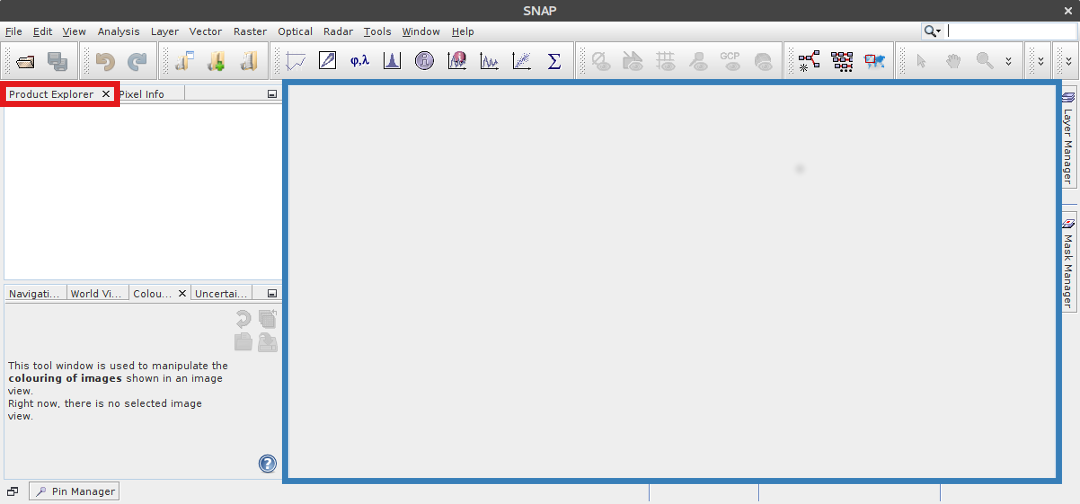
\includegraphics[width=0.6\textwidth]{fig:int.png}
    \caption{Interfaz gráfica del usuario. El área de visualización -en azul- con el \menu{Product Explorer} a la izquierda -en rojo-.}
    \label{fig:int}
\end{figure}

\section{Apertura de imágenes}

Desde el menú \menu{File>Open product...} abra la imagen
\begin{center} \directory{LC08\_224-078\_2018-01-05.dim}.
\end{center}
Haga doble click sobre el nombre de la imágen y se desplegará, en el \menu{Product Explorer} un árbol que incluye:
\\
\dirtree{%
    .1 [1] LC08\_224-078\_2018-01-05.
    .2 Metadata.
    .2 Vector Data.
    .2 Bands.
}

En esta cobertura encontramos

\begin{itemize}
    \item \emph{[1] LC08\_224-078\_2018-01-05}: El número de elemento entre corchetes, que marca en que orden se abrieron los productos y el nombre de la imagen.
    \item \emph{Metadata}: Los metadatos asociados a la imagen y su historial de procesamiento.
    \item \emph{Vector Data}: Los vectores contenidos dentro de la imagen.
    \item \emph{Bands}: Las bandas de la imagen y las operaciones de álgebra entre bandas.
\end{itemize}

\section{Visualización}

Es posible visualizar la imagen en color real. Para ello en el \menu{Product Explorer} seleccione \menu{Open RGB image windows} haciendo click derecho sobre el nombre de la imagen. Se desplegará una nueva ventana (Figura \ref{fig:RGB}) que le permitirá elegir la combinación de bandas. Por defecto aparecerá la combinación que utiliza las bandas \emph{red}, \emph{green} y \emph{blue} de \emph{Landsat-8}, desplieguela haciendo click en OK.

\begin{figure}[h!]
    \centering
    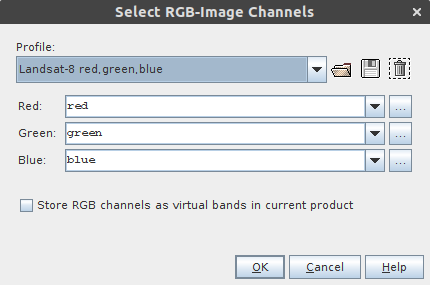
\includegraphics[scale=0.6]{fig:RGB.png}
    \caption{Ventana de combinación de bandas. Puede eligir una banda para cada canal del monitor (\emph{Red, Green, Blue}) o puede optar por una preseleccionada del menú \emph{Profile}}
    \label{fig:RGB}
\end{figure}

Explore la imagen utilizando las herramientas de navegación y zoom (Figura \ref{fig:mono})

\begin{figure}[h!]
    \centering
    \subfloat[]{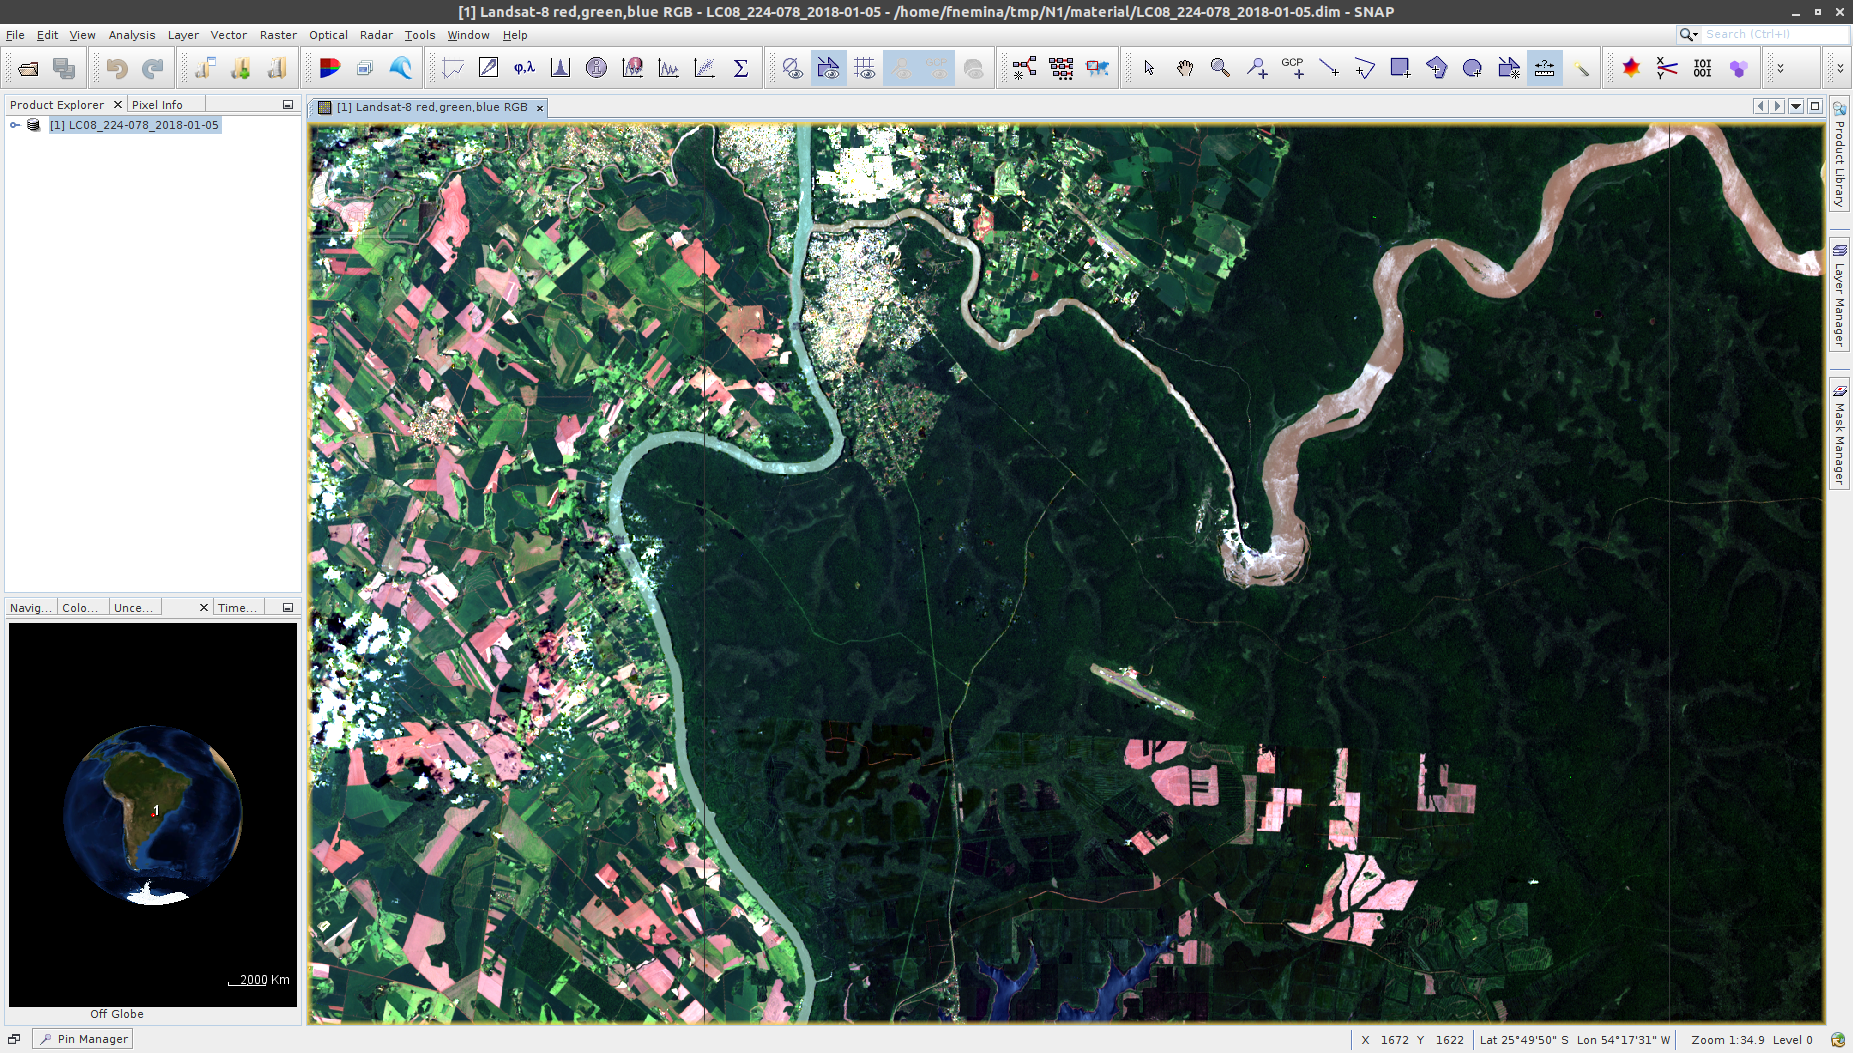
\includegraphics[width=0.6\textwidth]{fig:mono.png}}
    \\
    \subfloat[]{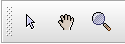
\includegraphics[scale=0.5]{fig:NAV.png}}
    \caption{Imagen desplegada en el visualizador. Herramientas de navegación. De izquierda a derecha: \menu{Selection tool}, para seleccionar objetos, \menu{Panning tool}, para moverse, y \menu{Zooming tool}, para hacer zoom.}
    \label{fig:mono}
\end{figure}

Localice dentro de la imagen el aeropuerto de cataratas del Iguazú.

\section{Mediciones}

Para medir la distancia entre dos puntos o a lo largo de una poligonal usando la herramienta \menu{Determines the distance between two points} (Figura \ref{fig:distancia}) que se encuentra en la barra de herramientas.

\begin{figure}[h!]
    \centering
    \subfloat[]{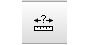
\includegraphics[scale=0.5]{fig:dico.png}}
    \\
    \subfloat[]{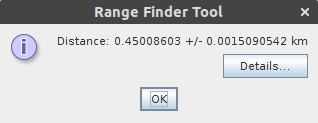
\includegraphics[width=0.3\textwidth]{fig:distancia.png}}
    \caption{Herramienta de medición de distancia \menu{Determines the distance between two points} y resultado de la medición.}
    \label{fig:distancia}
\end{figure}

Para utilizarla haga click sobre la herramienta y luego en un punto de la imagen para comenzar a medir. Dibuje una linea haciendo click en distintos puntos y finalice la medición haciendo doble click en el punto final. El largo de la poligonal y su error aparecerán en kilometros en una ventana emergente.

Mida la longitud de la pista de aterrizaje del aeropuerto de cataratas del Iguazú.

\section{Consulta de píxel}

Para obtener información sobre un pixel seleccione la pestaña \menu{Pixel info}, junto al \menu{Product explorer} (Figura \ref{fig:pixel}), y posicionese  sobre uno en la imagen.

\begin{figure}[h!]
    \centering
    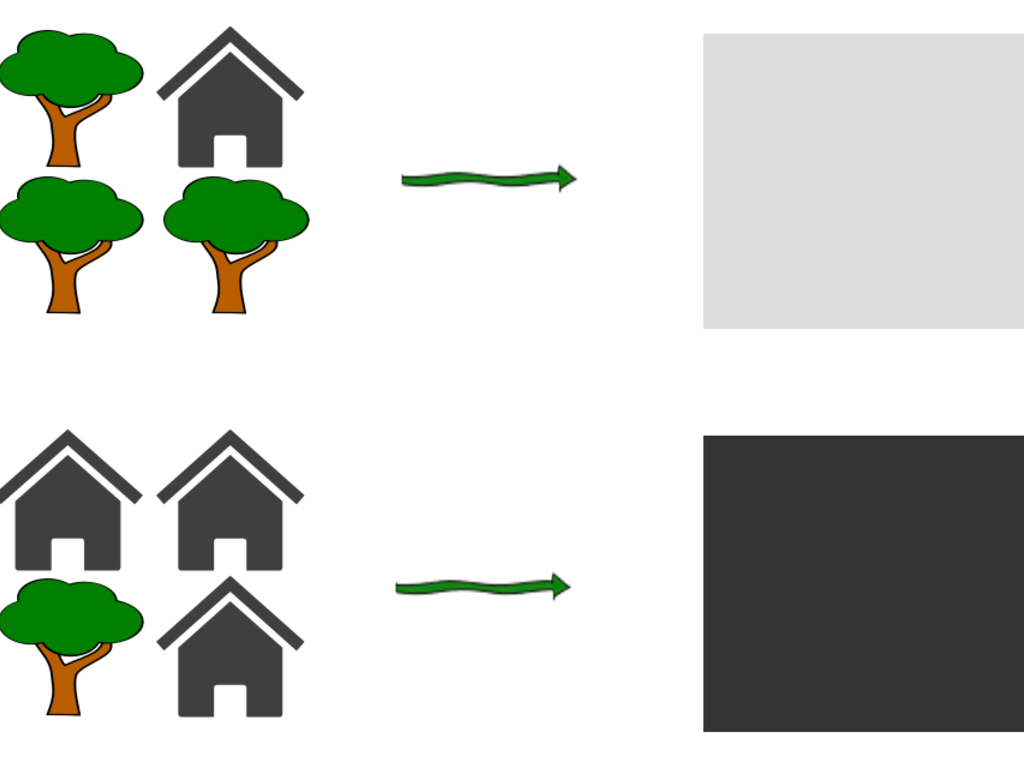
\includegraphics[width=0.3\textwidth]{fig:pixel.png}
    \caption{Herramienta de consulta de píxel. Puede verse la posición del píxel en la imagen, su latitud y longitud y el valor del píxel para la banda desplegada.}
    \label{fig:pixel}
\end{figure}

Allí encontrará la latitud y longitud, las coordenadas dentro del mapa y el valor del pixel en la banda abierta.

Halle las coordenadas en latitud y longitud de aeropuerto de cataratas del Iguazú.

\section{Multiples visualizadores}

Abra las imágenes
\begin{center} \directory{S2B\_MSIL2A\_2018-01-31.dim}.
\end{center}
y
\begin{center} \directory{MCD43A4.A2018039.h13v11.0065.dim}.
\end{center}

y desplieguelas en combinación de color RGB. Las tres corresponden a la misma zona durante el mes de enero de 2018.

Para ver las tres en simultaneo haga click en \menu{Window>Tile Horizontally} mostrandose de esa manera las imágenes vinculadas una junto a la otra. Moverse o hacer zoom en una imagen lo reproducirá en las otras. Para volver al modo habitual haga click en \menu{Window>Tile Single} (Figura \ref{fig:multiples}).

\begin{figure}[h!]
    \centering
    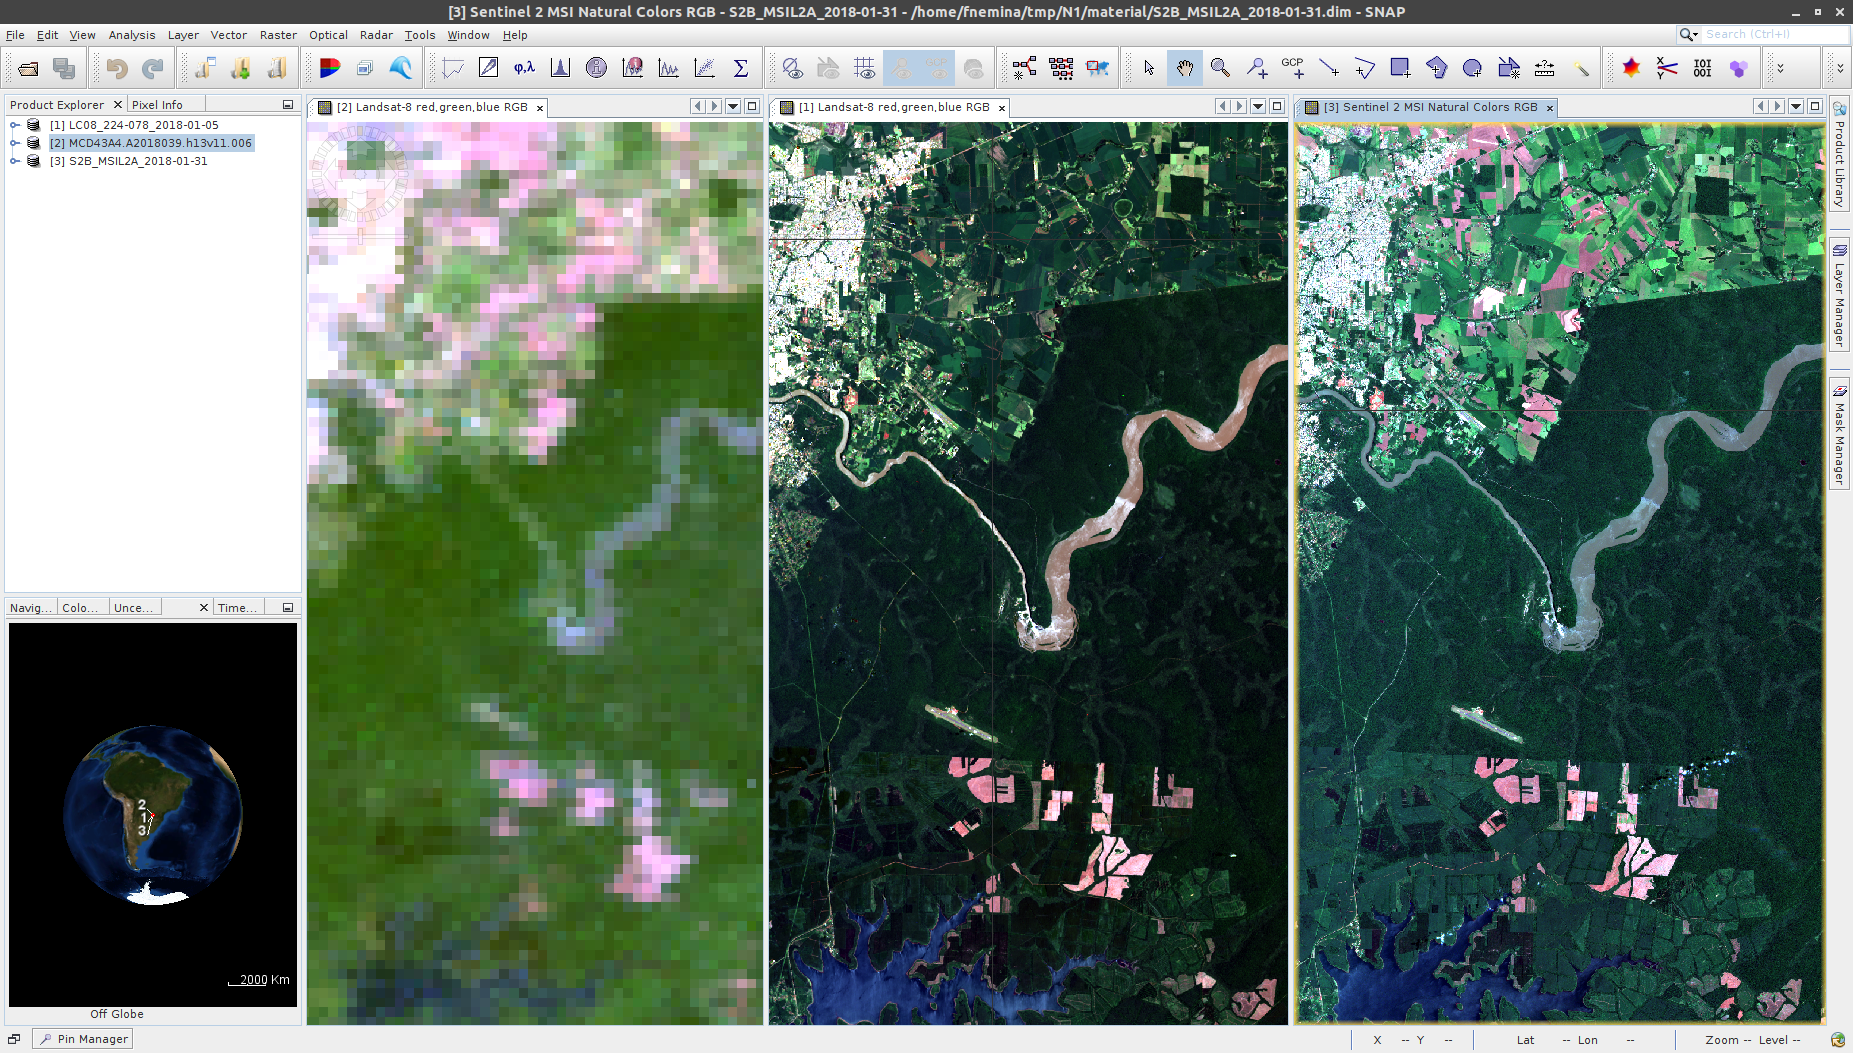
\includegraphics[width=0.6\textwidth]{fig:multiples.png}
    \caption{Distintas imágenes desplegadas en multiples visualizadores en simultaneo.}
    \label{fig:multiples}
\end{figure}

\section{Actividad práctica}

\begin{enumerate}
  \item Identifique en la imagen los siguientes objetos:
  \begin{enumerate}
    \item El río Iguazú que recorre la imagen de izquierda a derecha en color gris/marron.
    \item El río Paraná que corta la imagen de arriba a abajo celestre.
    \item La ciudad de Puerto Iguazú al sur-este del cruce de los rios Iguazú y Paraná.
    \item La zonas cultivadas al norte del río Iguazú con formas de parches en color verde.
    \item Laz onas cultivadas al oeste del río Paraná formadas por parches de color verde, con cultivo, y rosa, sin cultivo.
    \item La selva Paranaense al sur del río Iguazú en color verde.
    \item El embalse Urugua-í al sur de la imagen.
    \item La zona de forestaciones en color verde más oscuro entre la selva Paranaense y el embalse Urugua-í.
    \item El aeropuerto de cataratas del Iguazú en medio de la selva Paranaense.
  \end{enumerate}

  \item Mida dentro de las tres imágenes los siguientes objetos:
  \begin{enumerate}
    \item El largo de la pista de aterrizaje del aeropuerto.
    \item El ancho del río Paraná frente a la ciudad de Puerto Iguazú.
    \item El perímetro de la ciudad de puerto Iguazú.
    \item El perímetro del parche de selva Paranaense al norte del río Iguazú.
    \item El tamaño de un píxel.
  \end{enumerate}

  \item Identifique las coordenadas geográficas de los siguientes objetos:
  \begin{enumerate}
    \item El aeropuerto de las cataratas del Iguazú.
    \item La ciudad de Puerto Iguazú.
    \item La ciudad de Foz de Iguazú.
    \item Ciudad del este.
    \item La desembocadura del embalse Urugua-Í.
    \item El cruce entre los ríos Paraná y Iguazú.
    \item Las cataratas del Iguazú donde el río Iguazú se angosta.
  \end{enumerate}

\end{enumerate}
